\documentclass[11pt,a4paper, margin=1in]{article}
\usepackage{fullpage}
\usepackage{amsfonts, amsmath, pifont}
\usepackage{amsthm}
\usepackage{graphicx}
\usepackage{float}

\usepackage{tkz-euclide}
\usepackage{tikz}
\usepackage{pgfplots}
\pgfplotsset{compat=1.13}

\usepackage{geometry}
 \geometry{
 a4paper,
 total={210mm,297mm},
 left=10mm,
 right=10mm,
 top=10mm,
 bottom=20mm,
 }

 \author{
  Karaçanta, Kaan\\
  \texttt{e244854@metu.edu.tr}
}

\newcommand{\mySin}[1]{\textstyle\sin\left(#1\right)}
\newcommand{\myCos}[1]{\textstyle\cos\left(#1\right)}
\usepackage{hyperref}

\usepackage{inconsolata}
\usepackage{listings}
\usepackage{xcolor}
\usepackage[utf8]{inputenc}
\usepackage[T1]{fontenc}

\definecolor{codegreen}{rgb}{0,0.6,0}
\definecolor{codegray}{rgb}{0.5,0.5,0.5}
\definecolor{codepurple}{rgb}{0.58,0,0.82}
\definecolor{backcolour}{rgb}{0.95,0.95,0.92}

\lstdefinestyle{mystyle}{
    backgroundcolor=\color{backcolour},
    commentstyle=\color{codegreen},
    keywordstyle=\color{magenta},
    numberstyle=\tiny\color{codegray},
    stringstyle=\color{codepurple},
    basicstyle=\ttfamily\footnotesize,
    breakatwhitespace=false,
    breaklines=true,
    captionpos=b,
    keepspaces=true,
    numbers=left,
    numbersep=5pt,
    showspaces=false,
    showstringspaces=false,
    showtabs=false,
    tabsize=2
}

\lstset{style=myStyle}

\title{CENG 371 - Scientific Computing \\
Fall' 2024 - 2025 \\
Homework 1}

\begin{document}
\maketitle

\noindent\rule{19cm}{1.2pt}

% f(x) = (x * (((x+1)/x) - 1)) - 1
\section*{Question 1}

\begin{enumerate}
    % the plot of the function
    \item The plot of the function \( g(n) = f(n) / \epsilon \) is given below, where \( \epsilon = 10^{-6} \).
    \begin{figure}[H]
        \centering
        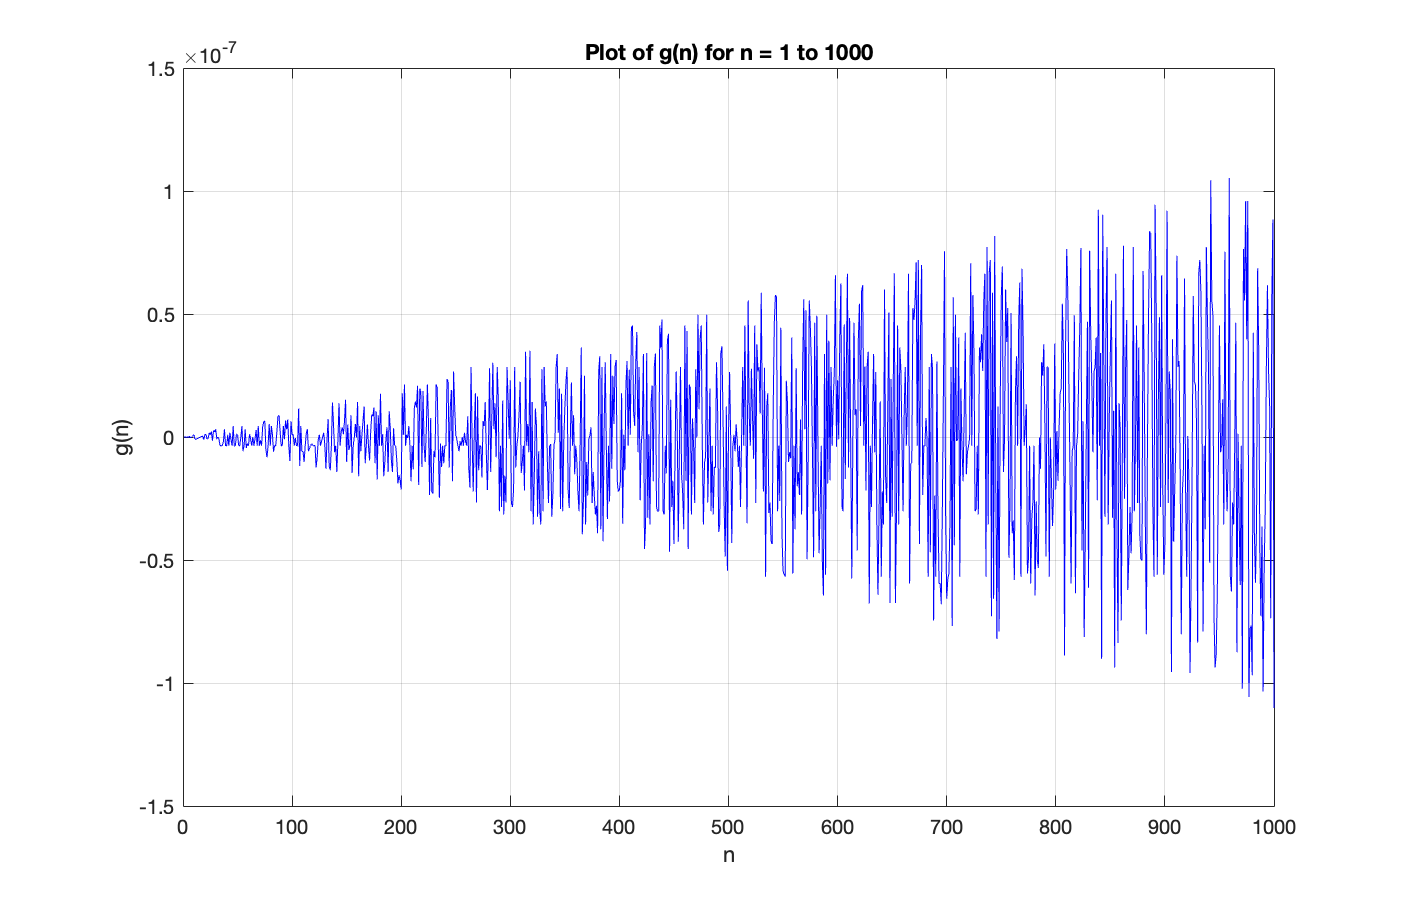
\includegraphics[width=0.9\textwidth]{q1.png}
        \caption{The plot of \(g(n)\)}
    \end{figure}

    % Which of the values of n satisfy g(n) = 0?
    \item The values of n where \( g(n) = 0 \) are \( 1, 2, 4, 8, 16, 32, 64, 128, 256, 512 \). In other words, \( g(n) = 0 \) when \(n\) is a power of 2. 
    
    % Explain why g(n) ̸= 0 of majority of n.
    \item 
    
    % g(n) seems to grow in size. Why?
    \item 

\end{enumerate}

\section*{Question 2}

\begin{enumerate}

    \item 

    \item

    \item

    \item

    \item

\end{enumerate}

\end{document}